\documentclass[12pt]{article}
\usepackage[margin=1in]{geometry}
\usepackage[pdftex]{graphicx}
\usepackage{amsmath,amssymb,amsthm}
\usepackage{float}
\usepackage{custom}
\usepackage{tikz}

% color boxes
\usepackage[many]{tcolorbox}
\tcbuselibrary{theorems}
\newtcbtheorem{pssolution}{Solution}{colback=orange!10,colframe=orange!40!black,fonttitle=\bfseries,breakable,enhanced}{sn}
\tcbset{noparskip/.style={before={\par\pagebreak[0]\medskip\parindent=0pt},
after={\par\medskip}}}

% code for totaling up points 
\usepackage{totcount}
\newtotcounter{tpts}
\newtotcounter{cpts}
\newtotcounter{endpts}
\newcommand{\clearpts}{\addtocounter{tpts}{\value{cpts}} \setcounter{cpts}{0}}
\newcommand{\pts}[1]{\clearpts \setcounter{cpts}{#1}}
\newcommand{\totpts}{\setcounter{endpts}{\totvalue{tpts} + \totvalue{cpts}}\arabic{endpts}}

% formatting for problems and solutions
\definecolor{ptred}{rgb}{0.7,0.1,0.1}
\newcommand{\ptfmt}[1]{\textbf{\color{ptred}#1\color{black}}}
\definecolor{advblue}{rgb}{0.1,0.1,0.7}
\newcommand{\advanced}{\!\textbf{\color{advblue}[A]\color{black}}\ }

\newtheorem*{solution}{Solution}
\newtheorem*{answer}{Answer}

\makeatletter
\newtheoremstyle{mystyle}
{\topsep}               % space above
{\topsep}               % space below
{}                      % bodyfont
{}                      % indent
{\bfseries}             % headfont
{}                      % punctuation
{0.6em}                 % space after head
{\llap{[\ptfmt{\arabic{cpts}}]\hspace{.6em}}\thmname{#1}\thmnumber{ #2}\thmnote{\normalfont{ (#3)}}{\bfseries .}}  %theoremheadspec
\theoremstyle{mystyle}
\newtheorem{pproblem}{Problem}
\makeatother

% headers and footers
\usepackage{fancyhdr}
\pagestyle{fancy}
\lhead{\href{https://activities.tjhsst.edu/physics/index.html}{TJHSST Physics Team}}
\chead{}
\rhead{Forces Mock Test}
\lfoot{}
\cfoot{\thepage}
\rfoot{}
\renewcommand{\headrulewidth}{0.4pt}
\setlength{\headheight}{14pt}

\newcommand{\psettitle}[1]{
    \begin{center}
    \huge \textbf{#1}
    \end{center}
}

\linespread{1.03} % give a little extra room
\setlength{\parindent}{0.2in} % reduce paragraph indent a bit

% uncomment to hide solutions
% \usepackage{environ}
% \NewEnviron{hide}{}
% \let\solution\hide
% \let\endsolution\endhide
% \let\answer\hide
% \let\endanswer\endhide

% tikz setup
\usetikzlibrary{calc,angles,quotes}
\tikzstyle{arrow} = [thick,->,>=stealth]

\begin{document}

\psettitle{Forces Mock Test}

\noindent
This is a mock test created by the officers of TJHSST Physics Team to prepare for the Forces Test in AP Physics C: Mechanics.
The recommended amount of time to finish this test is 1 hour.

The number in red next to each question represents the amount of points the question is worth. There is a total of \ptfmt{\totpts} points. The test consists of 10 Multiple Choice questions and 2 Free Response questions. If you need clarification on any of the problems, please contact us at \href{mailto:tjhsstphysicsteam@sgmail.com}{tjhsstphysicsteam@gmail.com}.

Work carefully, and best of luck.

\newpage

\subsection*{10 MCQs}

\pts{2}
\begin{pproblem}
    Eric drives on a vertical loop-de-loop (circle in a vertical plane), but unknown to him, his vehicle is in neutral (so the wheels are free to move, and the engine supplies no power to the wheels). At the bottom of the loop Eric experiences a normal force of $N_b$, at the
    side of the loop he experiences a normal force of $N_s$, and at the top
    of the loop he experiences a normal force of $N_t$. Rank the magnitude of
    the normal forces.
    Assume Eric is driving fast enough to stay in contact with the track at all times and slow
    enough to avoid getting a ticket.

    \begin{enumerate}[label=(\Alph*)]
        \item $N_s\le N_b\le N_t$
        \item $N_b\le N_t\le N_s$
        \item $N_t < N_s < N_b$
        \item $N_s < N_t < N_b$
        \item $N_b = N_s = N_t$
        % todo add rest of options
    \end{enumerate}
\end{pproblem}
\begin{solution}
    Writing out $F=ma$ for the top and bottom of the loop gives us
    \begin{align*}
        N_t+g&=\dfrac{mv^2}{r}\\
        N_b-g&=\dfrac{m(v+\Delta v)^2}{r}
    \end{align*}
    where $\Delta v>0$ because Eric's velocity increases as he goes down the loop-de-loop.
    It follows that $N_t<N_b$.
    By continuity, $N_s$ must be in between $N_t$ and $N_b$, so the answer is
    \fbox{C: $N_t<N_s<N_b$}
\end{solution}


\pts{2}
\begin{pproblem}
    A 450 kg car makes a U-turn in the shape of a semi-circle with a radius of 7.2m at a steady rate of 19.3 m/s. What is the magnitude of the net force on the car? 
    \begin{enumerate}[label=(\Alph*)]
        \item $1.46 \times 10^4$ N
        \item $2.33 \times 10^4$ N
        \item $3.84 \times 10^4$ N
        \item $6.25 \times 10^4$ N
        \item $8.56 \times 10^4$ N
    \end{enumerate}
\end{pproblem}
\begin{solution}
    In the force-body diagram of the car, we see that the force of gravity and the normal force cancel each other out, so we are only concerned with centripetal acceleration. Using the formula $F_{c} = \dfrac{mv^2}{R}$, we find the net force to be \fbox{B: $2.33 \times 10^4$ N} 
\end{solution}

\pts{2}
\begin{pproblem}
    A block slides down a friction-less inclined plane in a time $t_1$.
    The inclined plane then begins to accelerate upwards with a magnitude $a$.
    Which of the following is true about the new time $t_2$ taken for the block
    to slide down the plane?
    \begin{enumerate}[label=(\Alph*)]
        \item $t_2=0$ if $a$ is big enough.
        \item $t_2 < t_1$
        \item $t_2 = t_1$
        \item $t_2 > t_1$
        \item There is not enough information to decide
    \end{enumerate}
\end{pproblem}

\begin{solution}
    The acceleration down the plane becomes $g\sin\theta+a\sin\theta,\;a>0$. Since $t\propto \frac1{\sqrt{g}}$,
    the time decreases so the answer is \fbox{B: $t_2<t_1$}.
    
    If you're unsure why it's a plus sign, think about how as you accelerate in a car you
    get thrown backwards.
\end{solution}

\pts{2}
\begin{pproblem}
    A block of mass $m$ slides down an inclined plane of angle $\theta$ and coefficient of kinetic friction $\mu$.
    Its acceleration has components $a_x$ and $a_y$ relative to the ground.
    What is the ratio $a_y/a_x$?

    \begin{enumerate}[label=(\Alph*)]
        \item $\sin\theta$
        \item $\cos\theta$
        \item $\tan\theta$
        \item $\mu\sin\theta$
        \item $\mu\cos\theta$
    \end{enumerate}
\end{pproblem}

\begin{solution}
    In order to stay on the inclined plane, the $x$ and $y$ position
    of the block are under the constraint $y=x\tan\theta$. Taking
    two derivatives and rearranging gives \[
        \tan\theta=\dfrac{a_y}{a_x}
    \] or \fbox{A: $\tan\theta$}.
\end{solution}

% Inspired by F=ma 2014 Q2
\pts{2}
\begin{pproblem}
    A block slides down a plane as shown in the figure below.

    \begin{figure}[H]
        \centering
        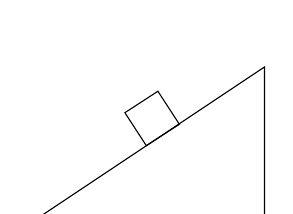
\begin{tikzpicture}
            \draw (0,0)-- (3, 0) -- (3, 2) -- cycle;
            \draw[rotate around={33:(3/2,1)}] (3/2,1) rectangle (2, 1.5);
        \end{tikzpicture}
    \end{figure}

    The coefficient of kinetic friction between the block and plane is $\mu$ such that $\mu < 1$. Which of the following shows the direction of the net force that
    the block exerts on the \textit{plane}?

    \begin{enumerate}[label=(\Alph*)]
        \item 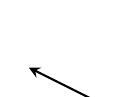
\begin{tikzpicture}
            \draw[arrow] (1,-0.5) -- (0, 0);
        \end{tikzpicture}
        \item \begin{tikzpicture}
            \draw[arrow] (1,0) -- (0, -0.5);
        \end{tikzpicture}
        \item \begin{tikzpicture}
            \draw[arrow] (0,0.5) -- (1, 0);
        \end{tikzpicture}
        \item 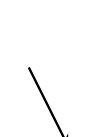
\begin{tikzpicture}
            \draw[arrow] (0,0.5) -- (0.5, -0.5);
        \end{tikzpicture}
        % This option might be a bit ambiguous?
        % \item \begin{tikzpicture}
        %     \draw[arrow] (0,0) -- (1, -0.5);
        % \end{tikzpicture}
        \item \begin{tikzpicture}
            \draw[arrow] (0,0) -- (0, -1);
        \end{tikzpicture}
    \end{enumerate}
\end{pproblem}

\begin{solution}
    The force on the planes on the plane includes the normal force pointing towards the inside of the plane, and the friction force pointing down the incline. The sum of these should point down and to the right, so the answer is \fbox{C}.
\end{solution}

\pts{2}
\begin{pproblem}
    An object of mass $m$ is attached to a rope of length $\ell$.
    The rope is attached to a pole, and rotates at an angular velocity $\omega$. What is the angle the rope makes with the horizontal?
    \begin{enumerate}[label=(\Alph*)]
        \item $\sin^{-1}\left(\dfrac{g}{\omega^2\ell}\right)$
        \item $\cos^{-1}\left(\dfrac{g}{\omega^2\ell}\right)$
        \item $\sin^{-1}\left(\dfrac{\omega^2\ell}{g}\right)$
        \item $\cos^{-1}\left(\dfrac{\omega^2\ell}{g}\right)$
        \item $\tan^{-1}\left(\dfrac{\omega^2\ell}{g}\right)$
    \end{enumerate}
\end{pproblem}
\begin{solution}
    The horizontal component of tension provides the centripetal force,
    and the vertical component balances the objects mass. Let $\theta$ be the angle with the horizontal. Then we have
    \begin{align*}
        T\cos\theta&=m\omega^2(\ell\cos\theta)\\
        T\sin\theta&=mg\\
        \implies \sin\theta&=\dfrac{g}{\omega^2\ell}\\
        \theta&=\sin^{-1}\left(\dfrac{g}{\omega^2\ell}\right)
    \end{align*}
    So the answer is \fbox{A}
\end{solution}

\pts{2}
\begin{pproblem}
    Ryan drives a car with mass m. He makes a turn in the shape of a quarter-circle of radius R with constant velocity $v$. The total frictional force acting on the car is $F$. Suppose Alex drives another car with mass M and makes the same turn traveling at a constant velocity of $2v$. Assume the only forces acting on the cars are gravity, normal force, and friction. You may neglect the mass of the driver, passengers, or items in the car. What is the magnitude and direction of the frictional force acting on Alex's car in terms of F, m, and/or M?
    \begin{enumerate}[label=(\Alph*)]
        \item $2F$ towards the center of the quarter-circle
        \item $4F$ away from the center of the quarter-circle
        \item $\frac{2Fm}{M}$ away from the center of the quarter-circle
        \item $\frac{2FM}{m}$ towards the center of the quarter-circle
        \item $\frac{4FM}{m}$ towards the center of the quarter-circle
    \end{enumerate}
\end{pproblem}
\begin{solution}
    The motion of the car while making this turn is uniform circular motion. Using the formula for centripetal acceleration, the acceleration on the first car is $a_1 = \frac{v^2}{R}$, and the acceleration on the second car is $a_2 = \frac{(2v^2)}{R} = \frac{4v^2}{R}$. Using F=ma, the centripetal forces on the first and second cars must be $\frac{mv^2}{R}$ and $\frac{4Mv^2}{R}$, respectively. Since gravity and the normal force act in the vertical direction, the frictional force must be equal to the centripetal force. Therefore, since the frictional force acting on the first car is defined as F,
    $$F = \frac{mv^2}{R}$$
    The force of friction acting on the second car must thus be:
    $$f = \frac{4Mv^2}{R} = \frac{4M}{m}\frac{mv^2}{R} = \frac{4FM}{m}$$
    Since the frictional force and centripetal force are equal, and centripetal force points towards the center of the circle in UCM, the frictional force points towards the center of the quarter-circle, so \boxed{E} is correct. 
\end{solution}

\pts{2}
\begin{pproblem}
    The frictionless pulley system with massless pulleys and very light rope shown below is used to lower a block at constant speed. The weight of the block shown is 120 N. What must be the magnitude of the external force $\Vec{F}$?
    \begin{figure}[H]
        \centering
        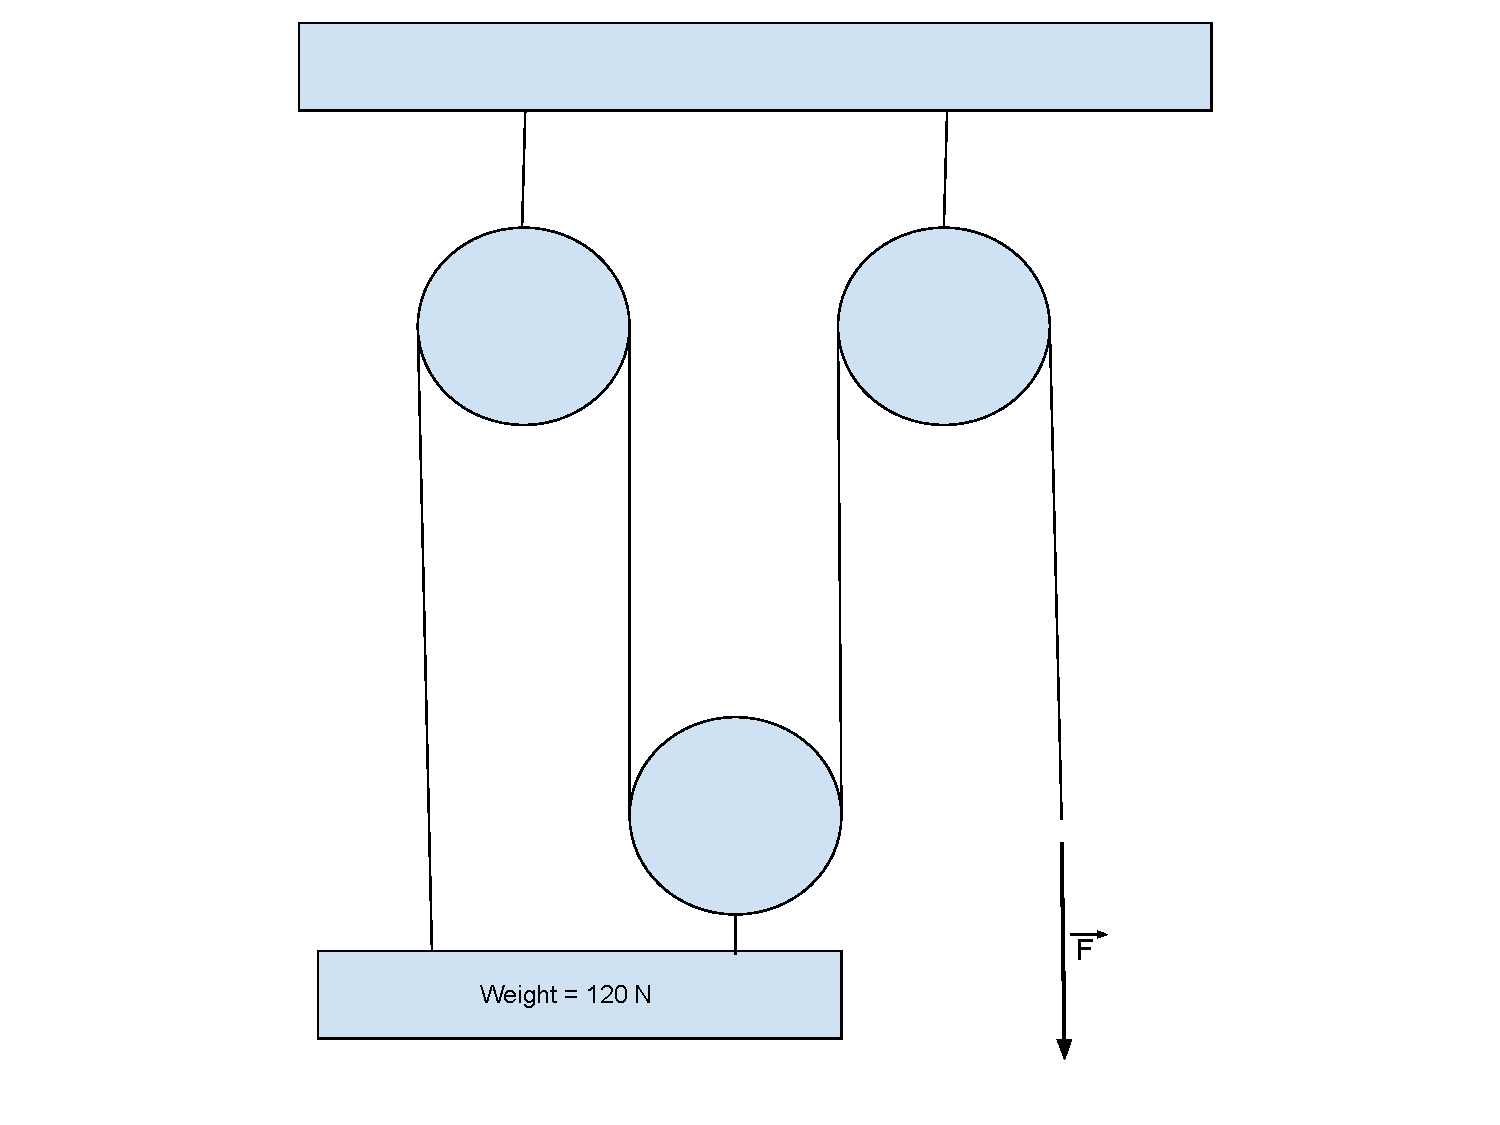
\includegraphics[scale=0.5]{PulleyDrawing2.pdf}
    \end{figure}
    \begin{enumerate}[label=(\Alph*)]
        \item $40$ N
        \item $60$ N
        \item $120$ N
        \item $180$ N
        \item $240$ N
    \end{enumerate}
    
    \begin{solution}
        First, note that a constant velocity implies an acceleration of zero.
        There are two ropes attached to the weight: one with
        tension $F$ and the other with tension $2F$. As such,
        we have \[
            F+2F-120\,\mathrm{N}=0
        \]
        so the answer is \fbox{A: F\,=\,40 N}
    \end{solution}
\end{pproblem}

\pts{2}
\begin{pproblem}
    Sophia pushes a 3.6 kg textbook with a horizontal force of 48 N on a flat table with coefficients of friction $\mu_s = 0.5$ and $\mu_k = 0.75$. What is closest to the magnitude of the total force the book exerts on the table?
    \begin{enumerate}[label=(\Alph*)]
        \item $40$ N
        \item $45$ N
        \item $48$ N
        \item $60$ N
        \item $63$ N
    \end{enumerate}
    \begin{solution}
        The two forces acting on the table are the normal force $N$ and the friction force $f=\mu_k N$.
        Note that it is kinetic friction because the force exceeds the maximum value of static friction.
        Since they are orthogonal, the magnitude of their sum can be computed with the Pythagorean theorem, which gives \[
            \left|\vec N+\vec f\right|=N\sqrt{1+\mu_k^2}
        \]
        From force balancing we have $N=mg$ so the magnitude is\[
            mg\sqrt{1+\mu_k^2}=\boxed{45\,\text{N}}
        \]
        or B.
    \end{solution}
\end{pproblem}

\pts{2} 
\begin{pproblem}
    A basketball of mass $M$ collides in the air with a tennis ball of mass $m$. During the collision, which of the following statements must be true? You may neglect the effects of gravity, since the time the collision takes is very small.
    \begin{enumerate}[label = \Roman*.]
        \item The average accelerations of the basketball and tennis ball are equal
        \item The average force exerted by the basketball on the tennis ball is equal to the average force exerted by the tennis ball on the basketball
        \item At some time during the collision, the net force acting on the basketball is equal to the net force acting on the tennis ball
    \end{enumerate}
    \begin{enumerate}[label=(\Alph*)]
        \item I only
        \item III only
        \item I and II
        \item II and III
        \item I, II, and III
    \end{enumerate}
    \begin{solution}
        Answer choices II and III are correct by Newton's Third Law.
        Answer I is incorrect, because the accelerations depend on the mass: $F=ma\implies a=F/m$.
        While $F$ may be the same, the mass $m$ differs between the basketball and tennis ball.
        Therefore, the answer is \fbox{D}
    \end{solution}
\end{pproblem}


\subsection*{2 Free Responses}
\setcounter{pproblem}{0}

\pts{10}
\begin{pproblem}
    Eric is illegally (he can't drive) taking Aarush on a road trip to touch some grass. On the way, they make a right onto a circular bank turn with an elevation angle of $\theta$. The distance between the driver's seat and shotgun is $d$, and the distance from Aarush to the center of the circle is $R$. Assume that the car is driving at the optimum banking angle.
    \begin{figure}[H]
        \centering
        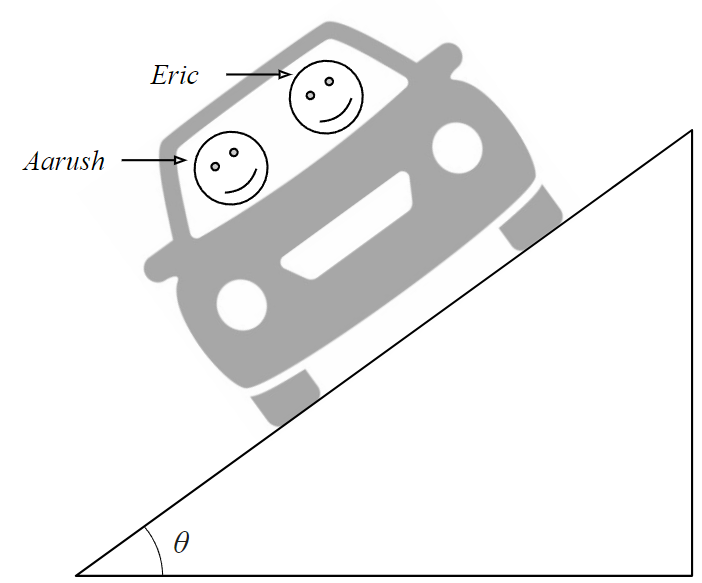
\includegraphics[scale=0.7]{BankTurn.png}
    \end{figure}
    
    \begin{enumerate}[label=\alph*)]
        \item Draw a Free Body Diagram of the car.
        \item What is the ratio of Eric's velocity to Aarush's in terms of $d$, $R$, and $\theta$?
        \item If Eric is driving at 12.9 m/s and the radius of the turn with respect to the \textbf{car} is 21.4 m, at what angle will the car experience zero frictional force?
    \end{enumerate}
\end{pproblem}

\begin{solution}
    \begin{enumerate}[label=\alph*)]
        \item Since the incline is at the optimum bank angle, there is no frictional force acting on the car. Additionally, the centripetal force is the $x$-component of the normal force, so it should not be noted as a separate force.
        \begin{figure}[H]
            \centering
            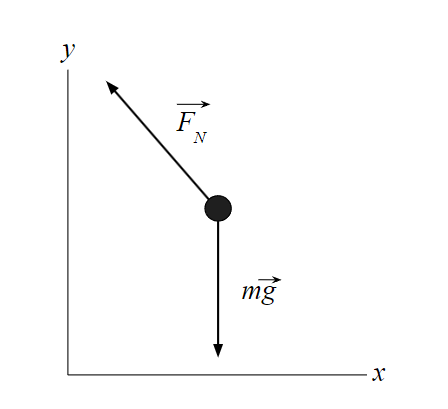
\includegraphics[scale=0.7]{BankFBD.png}
        \end{figure}
        \item 
        The only difference between Eric and Aarush is their distance from the center, or their respective radii. We use this to calculate their individual velocities. We know that the $y$-component of the normal force is equal to the gravitational force:
        \begin{align*}
            F_N\sin(90-\theta)&=mg\\
            F_N\cos\theta&=mg\\
            F_N&=\dfrac{mg}{\cos\theta}
        \end{align*}
        We know the $x$-component of the normal force is equal to the centripetal force. Given our original calculation for normal force, We find the velocity through the following:
        \begin{align*}
            F_N\cos(90-\theta)&=\dfrac{mv^2}{R}\\
            F_N\sin\theta&=\dfrac{mv^2}{R}\\
            \dfrac{mg}{\cos\theta}\sin\theta&=\dfrac{mv^2}{R}\\
            mg\tan\theta&=\dfrac{mv^2}{R}\\
            v&=\sqrt{gR\tan\theta}
        \end{align*}
        We see that the distances of Eric and Aarush from the center are $R + d\cos\theta$ and $R$ respectively, so we can plug these values into our equation for velocity and find the ratio.
        \begin{figure}[H]
            \centering
            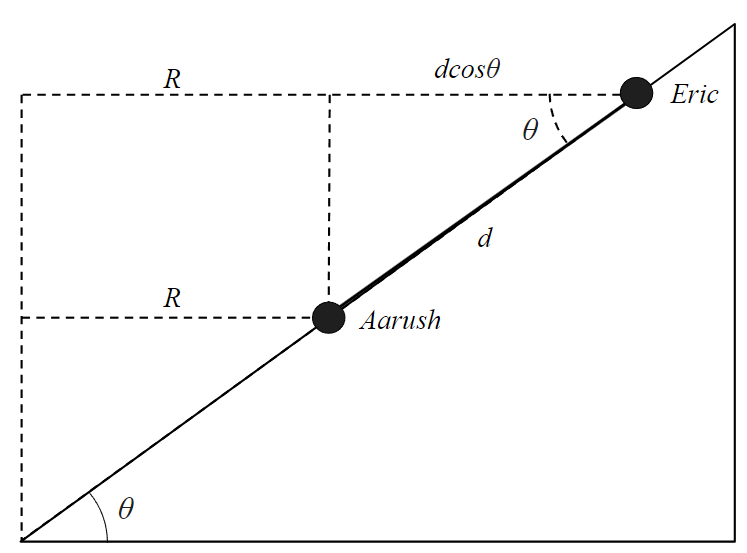
\includegraphics[scale=0.7]{BankPtB.png}
        \end{figure}
        \begin{center}
            $\dfrac{\sqrt{g(R+d\cos\theta)\tan\theta}}{\sqrt{gR\tan\theta}}$ =
            $\sqrt{\dfrac{R+d\cos\theta}{R}}$ =
            \fbox{$\sqrt{1+\dfrac{d\cos\theta}{R}}$}
        \end{center}
        \item The angle where no frictional forces are observed is the optimum angle, and we found the formula for velocity at this angle to be $v=\sqrt{gR\tan\theta}$. Rearranging this, we find 
        \[\theta = \tan^{-1}\left(\dfrac{v^2}{gR}\right) = \tan^{-1}\dfrac{(12.9)^2}{(9.8)(21.4)} \approx \fbox{$38.4^{\circ}$}\]
    \end{enumerate}
\end{solution}

\pts{10}
\begin{pproblem}
    An inclined plane of mass $m$ is stacked on top of an inclined plane
    of mass $M=2m$ (Figure \ref{frq1}). The coefficient of friction between
    them is $\mu_s=\mu_k\equiv\mu$.

    \begin{figure}[H]
        \centering
        \begin{tikzpicture}[scale=1.5]
            % lower triangle
            \coordinate (A) at (0,0);
            \coordinate (B) at (3,0);
            \coordinate (C) at (3,2);
            % upper triangle
            \coordinate (D) at (0.5, 1/3);
            \coordinate (E) at (2.5, 5/3);
            \coordinate (F) at (0.5, 5/3);
            
            \draw (A) -- (B) -- (C) -- cycle;
            \draw (D) -- (E) -- (F) -- cycle;

            \pic [draw, thick, -, "$\theta$", angle eccentricity=1.35, angle radius=10mm] {angle=B--A--C};
    
            % compute the centroid to place the text
            \node at ($1/3*($(A)+(B)+(C)$)$) {$M$};
            \node at ($1/3*($(D)+(E)+(F)$)$) {$m$}; 
            
            % ground
            \draw[thick] (-1,0) -- (4,0);
        \end{tikzpicture}
        \caption{Two blocks stacked}
        \label{frq1}
    \end{figure}

    \begin{enumerate}[label=\alph*)]
        \item Draw a Free Body Diagram for each inclined plane.
        \item What is the normal force between the bottom block and the floor?
    \end{enumerate}
\end{pproblem}

\begin{solution}
    We have the following free body diagrams. Note that by Newtons third law,
    the frictional force appears on both planes.

    \begin{figure}[H]
        \centering
        \begin{tikzpicture}
            % lower triangle
            \coordinate (A) at (4,0);
            \coordinate (B) at (7,0);
            \coordinate (C) at (7,2);
            \coordinate (X) at ($1/3*($(A)+(B)+(C)$)$);  % centroid
            % upper triangle
            \coordinate (D) at (-3.5, 1/3);
            \coordinate (E) at (-1.5, 5/3);
            \coordinate (F) at (-3.5, 5/3);
            \coordinate (G) at ($1/3*($(D)+(E)+(F)$)$);  % centroid

            % \draw (A) -- (B) -- (C) -- cycle;
            % \draw (D) -- (E) -- (F) -- cycle;
            \draw[fill=black] (G) circle (5pt) node[right,xshift=0.5em] {$m$};
            \draw [fill=black] (X) circle (5pt) node[right,xshift=0.5em] {$M$};

            % FBD upper
            \draw[arrow] (G) -- ($(G)-(0, 1.5)$) node[right] {$m\vec{g}$};
            \draw[arrow] (G) -- ($(G)+(-1, 3/2)$) node[left] {$\vec F_N$};
            \draw[arrow] (G) -- ($(G)+(2, 4/3)$) node[above] {$\vec F_f$};

            % FBD lower
            \draw[arrow] (X) -- ($(X)-(0, 1.5)$) node[below] {$M\vec{g}$};
            \draw[arrow] (X) -- ($(X)-(-1, 3/2)$) node[right] {$\vec F_N$};
            \draw[arrow] (X) -- ($(X)-(2, 4/3)$) node[above] {$\vec F_f$};
            \draw[arrow] (X) -- ($(X)+(0,2)$) node[left] {$\vec{F_N}_\text{ground}$};
        \end{tikzpicture}
        \caption{FBDs}
    \end{figure}

    To solve for the normal force between the ground and the bottom plane, consider the system
    of the bottom plane and the top plane together. This has a free body diagram that looks like
    this:
    \begin{figure}[H]
        \centering
        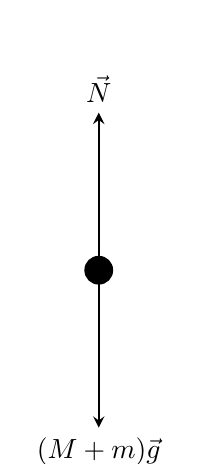
\begin{tikzpicture}
            \coordinate (C) at (0,0);
            \draw [fill=black] (C) circle (5pt);
            \draw[arrow] (C) -- ($(C)-(0, 2)$) node[below] {$(M+m)\vec g$};
            \draw[arrow] (C) -- ($(C)+(0, 2)$) node[above] {$\vec N$};
        \end{tikzpicture}
        \caption{Free Body Diagram of the $M+m$ system}
    \end{figure}

    Friction and the normal forces are then internal forces, so they cancel in pairs and we
    don't need to include them. From here, it's obvious that $N=(M+m)g$, so plugging
    in $M=2m$ gives us our solution of \fbox{$N=3mg$}.
\end{solution}

\end{document}